\subsection{Problem Statement}

We are given a multivariate time series $\mathcal{D} = \{(\mathbf{x}_t, y_t)\}_{t=1}^{T}$ from multiple sensors, where $\mathbf{x}_t \in \mathbb{R}^{n}$ denotes the $n$-dimensional measurement vector at time $t$:

\begin{equation}
\mathbf{X}_{\text{raw}} = \{\mathbf{x}_t\}_{t=1}^{T}, \quad 
\mathbf{x}_t = \big[x_{f1}(t),\; x_{f2}(t),\; \dots,\; x_{fn}(t)\big]^{\top} \in \mathbb{R}^{n}
\end{equation}

The goal is to detect anomalous windows while providing uncertainty estimates and feature-level explanations.

\subsubsection{Preprocessing: Windowing and Feature Engineering}

We first partition the continuous series into overlapping windows via sliding-window segmentation. This transforms $\mathcal{D}$ into windows of fixed length $W$, each analyzed for temporal correlations both individually and in relation to its neighbors. Feature extraction then enriches each window with temporal and statistical representations.

% \begin{figure*}[htbp]
% \centering
% \resizebox{\textwidth}{!}{%
% \begin{tikzpicture}[
%     node distance=1.5cm and 2cm, % lebih rapat
%     process/.style={rectangle, draw=black, thick, minimum width=2.2cm, minimum height=0.8cm, font=\small},
%     data/.style={trapezium, draw=black, thick, trapezium left angle=70, trapezium right angle=110, minimum width=2cm, minimum height=0.8cm, font=\small},
%     decision/.style={diamond, draw=black, thick, minimum width=2cm, minimum height=1cm, font=\small},
%     arrow/.style={->, thick}
% ]

% % Row 1: Data Processing
% \node[data, fill=inputcolor] (raw) {Raw Dataset};
% \node[process, fill=processcolor, right=of raw] (eng) {Feature\\Engineering};
% \node[process, fill=processcolor, right=of eng] (norm) {Normalization};
% \node[process, fill=processcolor, right=of norm] (window) {Windowing};

% % Row 2: Model
% \node[process, fill=tcncolor, below=1.5cm of window] (tcn) {Stochastic\\TCN};
% \node[process, fill=tcncolor, left=of tcn] (mc) {MC Dropout\\Inference};
% \node[data, left=of mc] (pred) {Predictions\\+ Uncertainty};

% % Row 3: Anomaly Detection
% \node[process, fill=anomalycolor, below=1.5cm of mc, xshift=-6.4cm] (error) {Error\\Calculation};
% \node[decision, fill=anomalycolor, right=of error] (thresh) {Threshold\\Check};
% \node[data, right=of thresh] (anomaly) {Anomaly\\Flags};

% % Connections
% \draw[arrow] (raw) -- (eng);
% \draw[arrow] (eng) -- (norm);
% \draw[arrow] (norm) -- (window);
% \draw[arrow] (window) -- (tcn);
% \draw[arrow] (tcn) -- (mc);
% \draw[arrow] (mc) -- (pred);
% \draw[arrow] (pred) -- (error);
% \draw[arrow] (error) -- (thresh);
% \draw[arrow] (thresh) -- (anomaly);

% % Feedback loop
% \draw[arrow, dashed, gray] (anomaly.north) -- ++(0,1) -| (tcn.south);

% \end{tikzpicture}%
% }
% \caption{End-to-End Stochastic TCN Anomaly Detection workflow}
% \label{fig:STCN_workflow}
% \end{figure*}

\begin{figure*}[!t]
    \centering
    % Make sure you have \usepackage{graphicx} in your preamble
    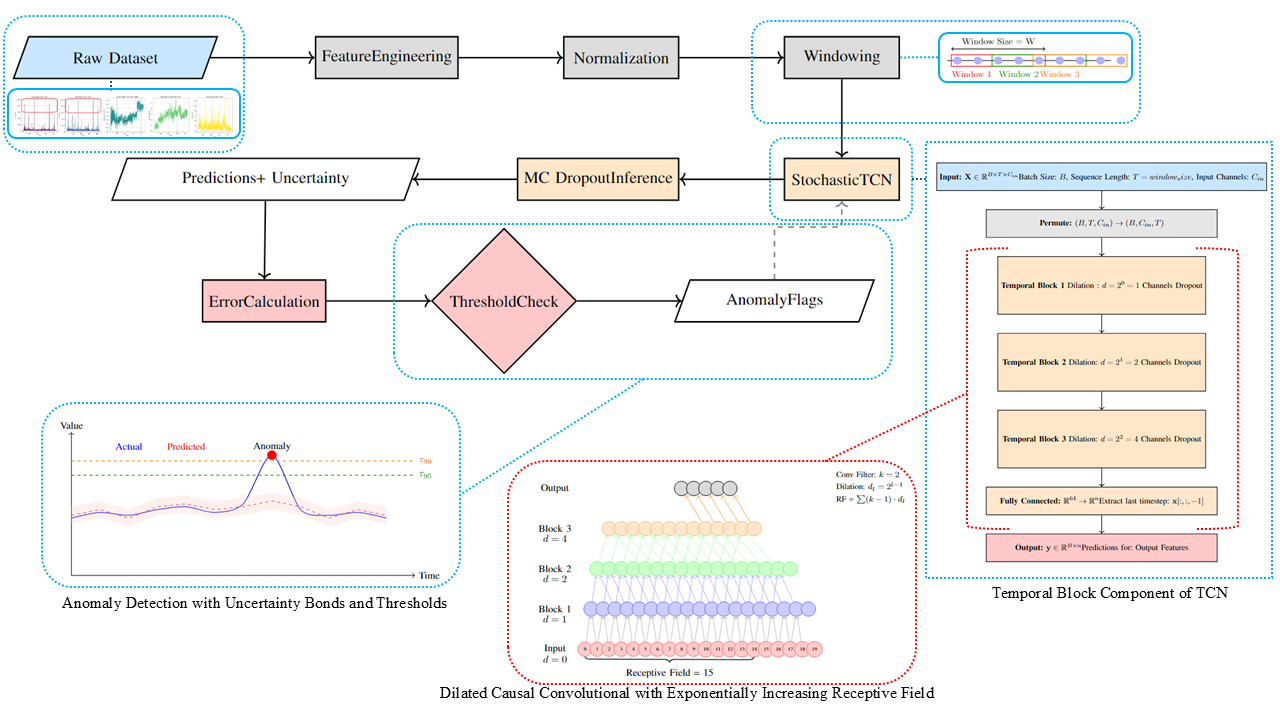
\includegraphics[width=\textwidth]{images/End to End Stochastic Workflow.png}
    \caption{End to End Stochastic TCN Anomaly Detection Workflow.}
    \label{fig:STCN_workflow}
\end{figure*}

\subsection{Enhanced TCN-Stochastic Architecture}

The proposed TCN-Stochastic Enhanced framework combines temporal convolutional networks with probabilistic modeling and three novel components: (1) Adaptive Uncertainty-Aware Attention (AUAA), (2) Dynamic Weight Adaptation for hybrid anomaly scoring, and (3) Feature-Level Anomaly Attribution.

\subsubsection{TCN Backbone with Stochastic Depth}

The backbone consists of three hierarchical temporal blocks (64 channels each) with exponentially increasing dilation rates $d \in \{1, 2, 4\}$. Each block stacks two dilated causal convolutions with weight normalization, ReLU activation, and dropout — serving dual purposes: regularization during training, and uncertainty quantification via Monte Carlo sampling at inference, following the Bayesian approximation framework of Gal and Ghahramani \cite{gal2016dropout_bayesian}.

\begin{algorithm}[H]
\footnotesize
\caption{TCN-Stochastic Model Training Procedure}
\label{alg:model_training}
\begin{algorithmic}
\Require Training dataset $\mathcal{D}_{train} = \{(\mathbf{x}_t, y_t)\}_{t=1}^{T_{train}}$, validation dataset $\mathcal{D}_{val}$, learning rate $\eta$, epochs $E$, batch size $B$, dropout rate $p_{drop}$, early stopping patience $P$
\Ensure Trained model parameters $\boldsymbol{\theta}^*$

\State \textbf{Initialization:}
\State Initialize model parameters $\boldsymbol{\theta}$ with He initialization
\State Set optimizer: Adam($\eta$)
\State Initialize best validation loss: $L_{best} \gets \infty$
\State Set patience counter: $patience \gets 0$

\For{epoch $e = 1$ to $E$}
    \State Shuffle training data
    \For{each mini-batch $(\mathbf{X}_b, \mathbf{y}_b)$ of size $B$}
        \State \textbf{Forward Pass:} $\hat{\mathbf{y}}_b \gets f_{\boldsymbol{\theta}}(\mathbf{X}_b)$
        \State \textbf{Loss Computation:}
        \State $L_{recon} \gets \mathcal{L}_{MSE}(\mathbf{y}_b, \hat{\mathbf{y}}_b) = \frac{1}{B} \sum_{i=1}^{B} \|y_i - \hat{y}_i\|^2$
        \State $L_{total} \gets L_{recon} + \lambda_{unc} \mathcal{L}_{uncertainty} + \lambda_{att} \mathcal{L}_{attention}$
        \State \textbf{Backward Pass:} $\nabla_{\boldsymbol{\theta}} L_{total} \gets \frac{\partial L_{total}}{\partial \boldsymbol{\theta}}$
        \State \textbf{Parameter Update:} $\boldsymbol{\theta} \gets \boldsymbol{\theta} - \eta \cdot \nabla_{\boldsymbol{\theta}} L_{total}$
    \EndFor
    
    \State \textbf{Validation:}
    \State $\hat{\mathbf{y}}_{val} \gets f_{\boldsymbol{\theta}}(\mathcal{D}_{val})$
    \State $L_{val} \gets \mathcal{L}_{MSE}(\mathbf{y}_{val}, \hat{\mathbf{y}}_{val})$
    
    \If{$L_{val} < L_{best}$}
        \State $L_{best} \gets L_{val}$
        \State Save model parameters: $\boldsymbol{\theta}^* \gets \boldsymbol{\theta}$
        \State $patience \gets 0$
    \Else
        \State $patience \gets patience + 1$
    \EndIf
    
    \If{$patience \ge P$}
        \State \textbf{Early stopping triggered}
        \State Break
    \EndIf
\EndFor

\State \textbf{Return} $\boldsymbol{\theta}^*$
\end{algorithmic}
\end{algorithm}

\begin{algorithm}[H]
\footnotesize
\caption{Monte Carlo Dropout Uncertainty Estimation}
\label{alg:mc_uncertainty}
\begin{algorithmic}
\Require Input $\mathbf{X} \in \mathbb{R}^{B \times T \times C}$, trained model $f_{\boldsymbol{\theta}}$, MC samples $N$, dropout rate $p_{drop}$
\Ensure Mean prediction $\bar{\mathbf{y}}$, uncertainty $\sigma$, 95\% confidence intervals

\State \textbf{Initialize:} Enable dropout at inference time
\State $\mathbf{Y}_{ens} \gets []$ \Comment{Collect $N$ stochastic forward passes}

\For{$n = 1$ to $N$}
    \State $\hat{\mathbf{y}}_n \gets f_{\boldsymbol{\theta}}(\mathbf{X})$ \Comment{Different dropout mask each pass}
    \State $\mathbf{Y}_{ens}.\text{append}(\hat{\mathbf{y}}_n)$
\EndFor

\State $\mathbf{P} \gets \text{stack}(\mathbf{Y}_{ens}) \in \mathbb{R}^{N \times B \times T \times C}$
\State $\bar{\mathbf{y}} \gets \text{mean}(\mathbf{P}, \text{dim}=0)$ \Comment{Empirical predictive mean}
\State $\sigma^2 \gets \text{var}(\mathbf{P}, \text{dim}=0)$ \Comment{Epistemic uncertainty}
\State $\sigma \gets \sqrt{\sigma^2}$

\State $\text{CI}_{95}^{\pm} \gets \bar{\mathbf{y}} \pm 1.96 \cdot \sigma$ \Comment{95\% confidence bounds}

\State \textbf{Return} $(\bar{\mathbf{y}},\, \sigma,\, \text{CI}_{95}^{\pm})$
\end{algorithmic}
\end{algorithm}
 

\textbf{Stochastic Depth.} We additionally apply stochastic depth \cite{huang_deep_2016}: each temporal block $l$ is randomly dropped during training with probability $p_l = 0.1 \cdot (l/L)$, where $L$ is the total number of blocks. This encourages redundant representations and improves generalization.

\subsubsection{Adaptive Uncertainty-Aware Attention (AUAA)}

Standard attention weights are computed from feature similarity alone, ignoring that predictions with high uncertainty may be unreliable. AUAA addresses this by modulating attention with predictive uncertainty.

\textbf{Formulation.} Given input $X \in \mathbb{R}^{B \times T \times C}$ and per-timestep uncertainty $\sigma_t \in \mathbb{R}$, the attention weights become:

\begin{equation}
\alpha_t = \text{softmax}\!\left(\frac{Q_t K_t^{\top}}{\sqrt{d_k}}\right) \odot \frac{1}{1 + \sigma_t}
\end{equation}

where $Q_t, K_t$ are query/key projections, $d_k$ is the key dimension, and $\odot$ denotes element-wise multiplication. The gate $g_t = 1/(1+\sigma_t)$ attenuates attention on uncertain timesteps, steering the model toward reliable patterns.

\textbf{Implementation.} AUAA uses 4-head attention with hidden dimension 64. The gate is learnable:
\begin{equation}
g_t = \sigma\!\left(W_g \cdot \sigma_t + b_g\right)
\end{equation}
where $\sigma(\cdot)$ here denotes the sigmoid function. This lets the network learn an optimal mapping from uncertainty to attention modulation.

\begin{algorithm}[H]
\footnotesize
\caption{Adaptive Uncertainty-Aware Attention (AUAA)}
\label{alg:auaa}
\begin{algorithmic}
\Require Input $\mathbf{X} \in \mathbb{R}^{B \times T \times C}$, uncertainty $\boldsymbol{\Sigma} \in \mathbb{R}^{B \times T}$, heads $H=4$, hidden dim $d=64$
\Require Projections $\mathbf{W}_Q^h, \mathbf{W}_K^h, \mathbf{W}_V^h$, gate params $\mathbf{W}_g, b_g$
\Ensure Uncertainty-modulated output $\mathbf{Y} \in \mathbb{R}^{B \times T \times C}$

\State \textbf{Step 1: Multi-head projections} ($d_k = d_v = d/H$)
\For{$h = 1$ to $H$}
    \State $\mathbf{Q}^h \gets \mathbf{X} \mathbf{W}_Q^h$, \quad $\mathbf{K}^h \gets \mathbf{X} \mathbf{W}_K^h$, \quad $\mathbf{V}^h \gets \mathbf{X} \mathbf{W}_V^h$
\EndFor

\State \textbf{Step 2: Standard scaled dot-product attention}
\For{$h = 1$ to $H$}
    \State $\mathbf{A}^h_{raw} \gets \frac{\mathbf{Q}^h (\mathbf{K}^h)^{\!\top}}{\sqrt{d_k}}$
    \State $\mathbf{A}^h \gets \text{softmax}(\mathbf{A}^h_{raw},\ \text{dim}=T)$
\EndFor

\State \textbf{Step 3: Uncertainty gate}
\State $\mathbf{g} \gets \sigma(\mathbf{W}_g \odot \boldsymbol{\Sigma} + b_g)$ \Comment{Learnable gate, $\sigma =$ sigmoid}

\State \textbf{Step 4: Uncertainty-modulated attention}
\For{$h = 1$ to $H$}
    \For{$t = 1$ to $T$}
        \State $\mathbf{A}^h[t,:] \gets \mathbf{A}^h[t,:] \odot \mathbf{g}[:,t]$
        \State $\mathbf{A}^h[t,:] \gets \frac{\mathbf{A}^h[t,:]}{\sum_j \mathbf{A}^h[t,j]}$ \Comment{Renormalize}
    \EndFor
\EndFor

\State \textbf{Step 5: Output}
\For{$h = 1$ to $H$}
    \State $\mathbf{O}^h \gets \mathbf{A}^h \mathbf{V}^h$
\EndFor
\State $\mathbf{O} \gets \text{Concat}(\mathbf{O}^1, \dots, \mathbf{O}^H)$
\State $\mathbf{Y} \gets \mathbf{O} \mathbf{W}_O$

\State \textbf{Return} $\mathbf{Y}$
\end{algorithmic}
\end{algorithm}


\subsubsection{Dynamic Weight Adaptation for Hybrid Scoring}

Conventional stochastic methods combine reconstruction error and uncertainty with fixed weights. In practice, the balance should shift: reconstruction error is more informative during stable operation, while uncertainty matters more under sensor degradation or high noise.

\textbf{Formulation.} Let $e_t$ be reconstruction error and $u_t$ be uncertainty at time $t$. The dynamic weight $\alpha_t$ is predicted as:

\begin{equation}
\alpha_t = \text{sigmoid}\!\left(W_\alpha \cdot [e_t,\, u_t,\, h_t] + b_\alpha\right)
\end{equation}

where $h_t$ encodes temporal context (GRU hidden state) and $[\cdot]$ denotes concatenation. The hybrid anomaly score blends the two signals:

\begin{equation}
s_t = \alpha_t \cdot e_t + (1 - \alpha_t) \cdot u_t
\end{equation}

with $\alpha_t \to 1$ favoring reconstruction error and $\alpha_t \to 0$ favoring uncertainty.

\textbf{Architecture.} Two encoder networks process error and uncertainty independently, a GRU captures temporal dynamics across windows, and a sigmoid output ensures $\alpha_t \in [0, 1]$.

\begin{algorithm}[H]
\footnotesize
\caption{Dynamic Weight Adaptation for Hybrid Anomaly Scoring}
\label{alg:dynamic_weight}
\begin{algorithmic}
\Require Reconstruction error $\mathbf{e} \in \mathbb{R}^{B \times T}$, uncertainty $\mathbf{u} \in \mathbb{R}^{B \times T}$, hidden state $\mathbf{h}_t \in \mathbb{R}^{d_h}$
\Require Encoder parameters $\mathbf{W}_e, b_e$, GRU parameters, weight adapter parameters $\mathbf{W}_\alpha, b_\alpha$
\Ensure Dynamic weight $\alpha_t \in [0,1]$ for each timestep $t$

\State \textbf{Step 1: Separate Encoding}
\State $\mathbf{z}_e \gets \sigma(\mathbf{W}_e \cdot \mathbf{e} + b_e) \in \mathbb{R}^{B \times T \times d_h}$
\State $\mathbf{z}_u \gets \sigma(\mathbf{W}_u \cdot \mathbf{u} + b_u) \in \mathbb{R}^{B \times T \times d_h}$
\State where $\sigma$ is the ReLU activation function

\State \textbf{Step 2: Concatenated Context Feature}
\State $\mathbf{c}_t \gets \text{Concat}(\mathbf{z}_{e,t}, \mathbf{z}_{u,t}) \in \mathbb{R}^{B \times 2d_h}$

\State \textbf{Step 3: Temporal Context Modeling with GRU}
\For{timestep $t = 1$ to $T$}
    \State $\mathbf{h}_t \gets \text{GRU}(\mathbf{c}_t, \mathbf{h}_{t-1})$
    \State \textbf{where:}
    \State $\quad \mathbf{r}_t \gets \sigma(\mathbf{W}_{ir} \mathbf{c}_t + \mathbf{W}_{hr} \mathbf{h}_{t-1} + b_r)$ (reset gate)
    \State $\quad \mathbf{z}_t \gets \sigma(\mathbf{W}_{iz} \mathbf{c}_t + \mathbf{W}_{hz} \mathbf{h}_{t-1} + b_z)$ (update gate)
    \State $\quad \tilde{\mathbf{h}}_t \gets \tanh(\mathbf{W}_{ih} \mathbf{c}_t + \mathbf{W}_{hh} (\mathbf{r}_t \odot \mathbf{h}_{t-1}) + b_h)$ (candidate)
    \State $\quad \mathbf{h}_t \gets (1 - \mathbf{z}_t) \odot \mathbf{h}_{t-1} + \mathbf{z}_t \odot \tilde{\mathbf{h}}_t$ (hidden state)
\EndFor

\State \textbf{Step 4: Dynamic Weight Prediction}
\For{timestep $t = 1$ to $T$}
    \State $\mathbf{f}_t \gets \text{Concat}(\mathbf{e}_t, \mathbf{u}_t, \mathbf{h}_t) \in \mathbb{R}^{B \times (2 + d_h)}$
    \State $\alpha_{raw,t} \gets \mathbf{W}_\alpha \cdot \mathbf{f}_t + b_\alpha$
    \State $\alpha_t \gets \text{sigmoid}(\alpha_{raw,t}) = \frac{1}{1 + e^{-\alpha_{raw,t}}}$
    \State ensures $\alpha_t \in [0, 1]$
\EndFor

\State \textbf{Step 5: Hybrid Anomaly Score Computation}
\State $\mathbf{s}_t \gets \alpha_t \odot \mathbf{e}_t + (1 - \alpha_t) \odot \mathbf{u}_t$
\State where higher $\alpha_t$ emphasizes reconstruction error, lower $\alpha_t$ emphasizes uncertainty

\State \textbf{Return} $(\boldsymbol{\alpha}, \mathbf{s}) = \{\alpha_t, s_t\}_{t=1}^T$
\end{algorithmic}
\end{algorithm}

\subsubsection{Feature-Level Anomaly Attribution}

To make anomaly detection actionable, we need to know \emph{which} sensors triggered the alarm — not just \emph{that} an anomaly occurred.

\textbf{Learnable Importance.} The module computes per-feature importance weights:

\begin{equation}
w_f = \text{softmax}\!\left(V \cdot \tanh(W \cdot X + b)\right)
\end{equation}

where $X$ is the input feature vector and $W, V, b$ are learned. These weights are applied to per-feature reconstruction errors:

\begin{equation}
\text{error}_f^{\text{weighted}} = w_f \cdot \text{error}_f
\end{equation}

\textbf{Inter-Sensor Correlation.} A learned correlation matrix $C \in \mathbb{R}^{n \times n}$ captures known physical dependencies (e.g., temperature--humidity coupling). The transformed features $X_{\text{corr}} = X \cdot C$ inform the importance computation, so correlated sensors are considered jointly rather than independently.

\begin{algorithm}[H]
\footnotesize
\caption{Feature-Level Anomaly Attribution}
\label{alg:feature_attribution}
\begin{algorithmic}
\Require Input features $\mathbf{X} \in \mathbb{R}^{B \times T \times n}$, reconstruction errors $\mathbf{E} \in \mathbb{R}^{B \times T \times n}$
\Require Attribution parameters $\mathbf{W}, \mathbf{V}, b$, correlation matrix $\mathbf{C} \in \mathbb{R}^{n \times n}$
\Ensure Feature importance weights $\mathbf{w}_f \in \mathbb{R}^n$, weighted errors $\mathbf{E}_{weighted} \in \mathbb{R}^{B \times T \times n}$

\State \textbf{Step 1: Feature Correlation Learning}
\For{feature pair $(i, j)$ where $i, j \in \{1, \dots, n\}$}
    \State $\mathbf{C}_{ij} \gets \text{Correlation}(\mathbf{X}_{:,:,i}, \mathbf{X}_{:,:,j})$
    \State captures known dependencies between sensors (e.g., temperature-humidity)
\EndFor

\State \textbf{Step 2: Correlated Feature Transformation}
\State $\mathbf{X}_{corr} \gets \mathbf{X} \times \mathbf{C} \in \mathbb{R}^{B \times T \times n}$
\State accounts for inter-sensor relationships

\State \textbf{Step 3: Temporal Feature Aggregation}
\State $\mathbf{X}_{agg} \gets \text{Mean}(\mathbf{X}_{corr}, \text{dim}=T) \in \mathbb{R}^{B \times n}$
\State aggregates temporal dimensions for spatial feature analysis

\State \textbf{Step 4: Learnable Feature Importance Computation}
\For{each batch instance $b = 1$ to $B$}
    \State $\mathbf{h}_b \gets \tanh(\mathbf{W} \cdot \mathbf{X}_{agg,b,:} + b) \in \mathbb{R}^{d_h}$
    \State $\mathbf{s}_b \gets \mathbf{V} \cdot \mathbf{h}_b \in \mathbb{R}^{n}$
    \State $\mathbf{w}_b \gets \text{softmax}(\mathbf{s}_b) = \frac{e^{\mathbf{s}_{b,i}}}{\sum_j e^{\mathbf{s}_{b,j}}}$
    \State ensures $\sum_i \mathbf{w}_{b,i} = 1$ (probability distribution)
\EndFor

\State \textbf{Step 5: Cross-Batch Averaging}
\State $\mathbf{w}_{mean} \gets \frac{1}{B} \sum_{b=1}^{B} \mathbf{w}_b \in \mathbb{R}^{n}$
\State provides stable feature importance across the batch

\State \textbf{Step 6: Weighted Error Computation}
\For{feature $f = 1$ to $n$}
    \For{timestep $t = 1$ to $T$}
        \For{batch $b = 1$ to $B$}
            \State $\mathbf{E}_{weighted}[b,t,f] \gets \mathbf{w}_{mean}[f] \cdot \mathbf{E}[b,t,f]$
            \State upweights errors for high-importance features
            \State downweights errors for low-importance features
        \EndFor
    \EndFor
\EndFor

\State \textbf{Step 7: Feature-Specific Anomaly Flagging}
\For{feature $f = 1$ to $n$}
    \State $\mathbf{A}_f \gets \mathbb{1}[\mathbf{E}_{weighted}[:,:,f] > \tau_f]$
    \State where $\tau_f$ is the feature-specific threshold
\EndFor

\State \textbf{Step 8: Attribution Summary Computation}
\State \textbf{For deployment and monitoring:}
\State $\mathbf{attribution\_rank} \gets \text{argsort}(\mathbf{w}_{mean}, \text{descending})$
\State $\mathbf{contribution\_percentage}_i \gets \frac{\mathbf{w}_{mean,i} \cdot \sum_{t,b} \mathbf{E}[b,t,i]}{\sum_{f,t,b} \mathbf{E}[b,t,f]} \times 100\%$

\State \textbf{Return} $(\mathbf{w}_{mean}, \mathbf{E}_{weighted}, \mathbf{A})$
\end{algorithmic}
\end{algorithm}

\subsubsection{Theoretical Uncertainty Bounds}
We provide provable bounds on false positive rates for anomaly detection using concentration inequalities.

\begin{Theorem}
(Chebyshev-Based Threshold) For any random variable $X$ with mean $\mu$ and variance $\sigma^2$, the probability of observing a value more than $k$ standard deviations from the mean is bounded by:

\begin{equation}
P(|X - \mu| > k\sigma) \leq \frac{1}{k^2}
\end{equation}
\end{Theorem}

\textbf{Application to Anomaly Detection.} Given predicted uncertainties $\{u_t\}_{t=1}^T$, we compute a threshold $\tau$ that guarantees a false positive rate (FPR) of at most $\epsilon$:

\begin{equation}
\tau = \bar{u} + \sqrt{\frac{1}{\epsilon}} \cdot \sigma_u
\end{equation}

where $\bar{u}$ and $\sigma_u$ are the mean and standard deviation of predicted uncertainties. This provides a distribution-free guarantee on anomaly detection performance.

\textbf{Calibrated Confidence Intervals.} We also compute calibrated confidence intervals for predictions:

\begin{equation}
[\hat{y}_t - z_{1-\alpha/2} \cdot \sigma_t \cdot \lambda, \hat{y}_t + z_{1-\alpha/2} \cdot \sigma_t \cdot \lambda]
\end{equation}

where $z_{1-\alpha/2}$ is the standard normal quantile, $\sigma_t$ is the predicted standard deviation, and $\lambda$ is a learnable calibration scale parameter optimized during training.

\subsubsection{Dilated Causal Convolution}

Dilated causal convolutions are the core building block of TCNs \cite{mehta_nac-tcn_2023}. Causality is enforced by left-only padding, so predictions at time $t$ depend only on past and present inputs. Dilations insert gaps between filter taps, enabling the receptive field (RF) to grow exponentially with depth without increasing parameters or reducing resolution. For a kernel size $k$ and dilation $d_l$ at layer $l$, the per-layer receptive field contribution is $(k-1) \cdot d_l$, yielding a total RF of:

\begin{equation}
\text{RF} = \sum_{l=1}^{L} (k - 1) \cdot d_l
\end{equation}

In our architecture, $k=2$ and $d_l = 2^{\, l-1}$, giving $\text{RF} = 1 + 2 + 4 = 7$, which covers enough temporal context for short-to-medium-range dependencies.

\subsubsection{Anomaly Detection and Thresholding}

Reliable anomaly detection requires separating true anomalies from normal variation using well-calibrated thresholds. We implement four complementary strategies:

\begin{enumerate}
    \item \textbf{Percentile-based:} $\tau = Q_{0.95}(\{s_t\})$ — simple, non-parametric.
    \item \textbf{Adaptive:} $\tau = \tau_{\text{base}} \cdot (0.8 + 0.4 \cdot \bar{\alpha})$, where $\bar{\alpha}$ is the mean dynamic weight — thresholds tighten or relax based on model confidence.
    \item \textbf{Theoretical (Chebyshev):} $\tau = \bar{u} + \sqrt{1/\epsilon} \cdot \sigma_u$ — provides an FPR guarantee of at most $\epsilon$.
    \item \textbf{Distribution-free:} $\tau = Q_{1-\gamma}(\{s_t\})$, where $\gamma$ is the expected contamination ratio.
\end{enumerate}

\begin{align}
\tau_{95} &= Q_{0.95}\big(\{e_i(t) : \forall t \in \text{validation set}\}\big) \\
\tau_{99} &= Q_{0.99}\big(\{e_i(t) : \forall t \in \text{validation set}\}\big)
\label{fig:threshold}
\end{align}

\noindent\textbf{where:}
\begin{itemize}
    \item $\tau_{95}, \tau_{99}$ : threshold values at the 95th and 99th percentiles, respectively.
    \item $Q_{p}(\cdot)$ : quantile function at probability level $p$.
    \item $e_i(t)$ : reconstruction error (or prediction error) for instance $i$ at time $t$.
    \item $\text{validation set}$ : the dataset used to estimate thresholds, disjoint from the training set.
\end{itemize}

\vspace{6pt}
\noindent\textbf{Algorithm~1:} Stochastic TCN-based Anomaly Detection
\label{alg:stochastic_tcn}
\vspace{4pt}

\noindent \textbf{Input:} Trained TCN model $f_{\theta}$, input sequence $\mathbf{X}$, thresholds $\tau_{95}, \tau_{99}$\\
\textbf{Output:} Anomaly flags $\mathbf{A}_{95}, \mathbf{A}_{99}$

\medskip
\noindent \textbf{1. Monte Carlo Prediction:}\\
$\hat{\mathbf{y}}, \boldsymbol{\sigma} \gets \text{MC-Predict}(f_{\theta}, \mathbf{X}, N=50)$

\medskip
\noindent \textbf{2. Error Calculation:}\\
\textbf{for} each feature $i \in \{1,\dots,5\}$ \textbf{do}\\
\quad $e_i \gets |y_i - \hat{y}_i|$\\
\textbf{end for}

\medskip
\noindent \textbf{3. Anomaly Detection:}\\
\textbf{for} each feature $i$ and timestep $t$ \textbf{do}\\
\quad $\mathbf{A}_{95}[i,t] \gets \mathbf{1}_{[\,e_i(t) > \tau_{95}\,]}$\\
\quad $\mathbf{A}_{99}[i,t] \gets \mathbf{1}_{[\,e_i(t) > \tau_{99}\,]}$\\
\quad \textbf{if} $e_i(t) > \hat{y}_i(t) + 2\sigma_i(t)$ \textbf{then}\\
\quad\quad Mark as high-confidence anomaly\\
\quad \textbf{end if}\\
\textbf{end for}

\medskip
\noindent \textbf{return} $\mathbf{A}_{95}, \mathbf{A}_{99}$
\vspace{6pt}


Algorithm~\ref{alg:stochastic_tcn} summarizes the detection procedure: Monte Carlo predictions yield mean $\hat{\mathbf{y}}$ and uncertainty $\sigma$, reconstruction error $e_i = |y_i - \hat{y}_i|$ is compared against thresholds $\tau_{95}, \tau_{99}$, and points exceeding $\hat{y} + 2\sigma$ are flagged as high-confidence anomalies.